%% LyX 2.3.6 created this file.  For more info, see http://www.lyx.org/.
%% Do not edit unless you really know what you are doing.
\documentclass[a4paper,english]{scrartcl}
\usepackage[T1]{fontenc}
\usepackage[latin9]{inputenc}
\usepackage{url}
\usepackage{graphicx}

\makeatletter

%%%%%%%%%%%%%%%%%%%%%%%%%%%%%% LyX specific LaTeX commands.
\pdfpageheight\paperheight
\pdfpagewidth\paperwidth


\makeatother

\usepackage{babel}
\usepackage{listings}
\renewcommand{\lstlistingname}{Listing}

\begin{document}
\title{SEA3004F M2P1: Properties of the atmosphere}
\author{Ocean and Atmosphere Dynamics}
\date{Module 2}
\maketitle

\section{The standard atmosphere}

The US Standard Atmosphere (1976) is a series of models that define
values for atmospheric temperature, density, pressure, and other properties
over a wide range of altitudes. A MATLAB/octave \textbf{script} is
freely available here\url{http://www.mathworks.com/matlabcentral/fileexchange/28135-stdatmo--standard-atmosphere-function}.
In the assignment, we will use a simplified version of this script
that returns temperature values given the geometric altitude. 
\begin{enumerate}
\item Create a folder M2P1 on the computer
\item Download the scripts in that directory. (make sure they are moved
to the M2P1 directory)
\item Launch the software and change folder to M2P1 as done for the previous
practical
\end{enumerate}
We will practice the function by plotting the atmospheric temperature values up to the mesopause (\textasciitilde 80 km):

\begin{lstlisting}[language=Matlab,basicstyle={\small},showstringspaces=false,frame=lines]
>> help tstdatm      % first check which are the inputs to the function
>> z = 0:1000:80000; % create the input array to the function, 
                     % altitude (in metres) in steps of 1 km
>> T = tstdatm(z);   % compute the temperature and assign it to a
                     % local array called T (in K)
>> figure
>> plot(T,z) % the plot function takes at least 2 arguments plot(x,y)
>> xlabel('Temperature [K]')
>> ylabel(Altitude [m]')
>> print -dpng temp_STDATM.png
\end{lstlisting}


\section{Creating functions}

A function in computer programming is a subprogram or procedure: a
block of statements identified by a special ``header'' that accepts
an input (or more inputs) and produces an output. Functions that are
not built-in (i.e. the math functions sin, cos, etc.) are usually
called ``scripts'', because they are in separate files.

A function has a list of arguments: the inputs and the outputs. The
name of the file matches the name of the function, and when ``called''
from the command line, the interpreter passes the list of inputs to
the function through a process called \emph{referencing}, and the
function returns the output. 

\begin{figure}
\begin{centering}
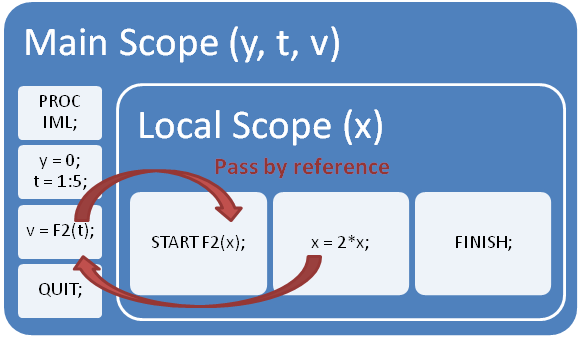
\includegraphics[width=6cm]{scope}
\par\end{centering}
\caption{The scope of variables in the main program (your workspace in octave)
and in a function}

\end{figure}

We shall now practice the creation of a function and its use by passing
variables from the main scope to the function, and back to the workspace:

\begin{lstlisting}[language=Matlab,basicstyle={\small},showstringspaces=false,frame=lines]
>> edit xsquared.m   % creates a new file and opens the editor

function y = xsquared (x)
% this function computes the square of a number
y = x.^2;
end

>> xsquared(2)

>> x = 1:10; 
>> xsquared(x)

>> figure 
>> plot(x,xsquared(x),'-o')
\end{lstlisting}


\section{Exercise 1: Approximated saturation vapor pressure {[}20{]}}

The saturation vapor pressure can be computed with the Clausius-Clapeyron
equation. In the lecture notes, we have introduced an approximated
form, 
\[
e_{s}=Ae^{\beta T}
\]
with A=6.11 hPa; $\beta$=0.067 $^{\circ}$C. In this exercise, you
will create a \textbf{function} (a script that accepts arguments and
creates output values) to calculate it automatically.
\begin{enumerate}
\item Create a new script called \texttt{svpa.m} (saturation vapor pressure
\emph{approximated}) using the command \texttt{edit svpa.m.} Write
the code found in the inset below to compute $e_{s}$ in Pa given
temperature in K. \textbf{DO NOT COPY AND PASTE BECAUSE YOU WILL ADD
SPECIAL INVISIBLE CHARACTERS AND THE CODE WILL NOT RUN!} Copy the
code exactly as it is and think about what you write. Please note
the use of \texttt{'. *'} as the multiplication operator,
which stands for element-by-element multiplication in matlab
syntax.
\begin{lstlisting}[language=Matlab,basicstyle={\small},showstringspaces=false,frame=lines]
function es = svpa(tempK)
% SVPA Saturation Vapour Pressure (Approximated solution)
%   es = svpa(temp)
%   temp: temperature array in degrees K
%   es: pressure in Pa

% constants
A=6.11e2;    % Pa 
beta=0.067;  % 1/degC

% convert from K to degC
tempC = tempK-273.15;
es = A.*exp(beta.*tempC);

endfunction
\end{lstlisting}
\item Write the code to generate a temperature array with values between
-2 and 40 $^{\circ}C$ in steps of 1 $^{\circ}C$, which will be the
input to your function. 
\begin{enumerate}
\item Plot the saturation vapor pressure for that range of temperature
values 
\item Add a title and the correct axes labels
\end{enumerate}
\end{enumerate}

\section{Exercise 2: Water vapor in the standard atmosphere {[}50{]}}

You will use your approximated function to calculate the saturation
vapor pressure as a function of the temperature T and the equation of
state of water vapor, 
\[
e=\rho_{v}R_{v}T.
\]
The value of the constants should be taken from the lecture notes.
The temperature values for the various altitudes can be computed from
the standard atmosphere \texttt{tsdtam} function presented in the
tutorial. 
\begin{enumerate}
\item Write the code to compute the maximum amount of water vapour per unit
volume that air can hold 
\begin{enumerate}
\item at the surface, and 
\item at the height of 10 km. \textbf{Note}: the code must be commented on
and variables or named constants indicated with their appropriate units.
\end{enumerate}
\item Write the code to 
\begin{enumerate}
\item Create a figure showing the saturation vaporpressure as a function
of altitude, using the standard atmosphere temperature from the surface
to the altitude of 20 km in steps of 500 m as input. Give the units
of the Y-axis in km and the units of the X-axis in hPa. 
\item Compare the result with the complete version of the Clausius-Clapeyron
equation proposed by Goff and Gratch (1946) found in file
\texttt{svp.m}. The graphs of both functions (\texttt{svp} and \texttt{svpa})
\textbf{must be shown on the same figure} and the legend must identify
the lines (hint: to add another line and the legend, see the code
snippet below).
\begin{lstlisting}[language=Matlab,basicstyle={\small},showstringspaces=false,frame=lines]
% HINT: HOW TO ADD 2 LINES ON A PLOT
>> plot(x1,y1,'k-')
>> hold on  % this command turns on 'holding' previous lines
>> plot(x2,y2,'r--')
>> legend('Description 1','Description 2')
\end{lstlisting}
\end{enumerate}
\end{enumerate}

\section{How to present the results}

Submit the livescript named \texttt{M2P1\_STUDENT\_NUMBER.mlx} containing
one section for each exercise, \textbf{and} any other script needed
to run the code. \textbf{VERY IMPORTANT}: Make sure that the script
contains comments explaining what the various statements do, as well
as the units of constants and variables.
\end{document}
